\documentclass{article}

% content/resources/templates/preamble.tex
\usepackage[margin=0.6in]{geometry}
\author{Milav Dabgar}
\usepackage{amsmath,amssymb,amsthm}
\usepackage{booktabs}
\usepackage{multirow}
\usepackage{xcolor}
\usepackage{tcolorbox}
\tcbuselibrary{breakable,skins}
\usepackage[colorlinks=true,linkcolor=blue]{hyperref}
\usepackage{titlesec}
\usepackage{enumitem}
\usepackage{tikz}
\usepackage{pgfplots}
\usepackage{circuitikz}
\usepackage[version=4]{mhchem}
\usepackage{longtable}
\usepackage{array}
\usepackage{float}
\usepackage{caption}
\usepackage{listings}

\lstset{
  basicstyle=\small\ttfamily,
  breaklines=true,
  breakatwhitespace=false,
  postbreak=\mbox{\textcolor{red}{$\hookrightarrow$}\space},
  float=false,
  numbers=left,
  numberstyle=\tiny\color{gray},
  numbersep=10pt,
  xleftmargin=2em,
  keywordstyle=\color{blue},
  commentstyle=\color{green!60!black},
  stringstyle=\color{purple},
  backgroundcolor=\color{gray!5},
  showstringspaces=false,
  tabsize=2,
  captionpos=b,
  keepspaces=true,
  columns=flexible
}

\pgfplotsset{compat=1.18}
\usetikzlibrary{shapes,arrows,positioning,calc,patterns,decorations.pathmorphing,decorations.markings,arrows.meta}

% Color scheme
\definecolor{headcolor}{RGB}{0,102,204}
\definecolor{keycolor}{RGB}{220,20,60}
\definecolor{solutioncolor}{RGB}{34,139,34}
\definecolor{mnemoniccolor}{RGB}{148,0,211}
\definecolor{codecolor}{RGB}{0,0,100}

% Spacing
\setlength{\parskip}{3pt}
\setlist[itemize]{nosep}
\setlist[enumerate]{nosep}

% Title formatting
\titleformat{\section}{\Large\bfseries\color{headcolor}}{\thesection}{1em}{}
\titleformat{\subsection}{\large\bfseries\color{headcolor}}{\thesubsection}{1em}{}

% Pandoc tightlist compatibility
\providecommand{\tightlist}{%
  \setlength{\itemsep}{0pt}\setlength{\parskip}{0pt}}

% Pandoc longtable compatibility
\newcounter{none}
\def\thenone{}


% content/resources/templates/english-boxes.tex

% Custom environments
\newtcolorbox{solutionbox}{
 breakable,
 enhanced,
 colback=solutioncolor!5!white,
 colframe=solutioncolor!75!black,
 fonttitle=\bfseries,
 title=Solution
}

\newtcolorbox{solutionboxnobreak}{
 colback=solutioncolor!5!white,
 colframe=solutioncolor!75!black,
 fonttitle=\bfseries,
 title=Solution
}

\newtcolorbox{keyformula}{
 breakable,
 enhanced,
 colback=keycolor!5!white,
 colframe=keycolor!75!black,
 fonttitle=\bfseries,
 title=Key Formula
}

\newtcolorbox{mnemonicboxenv}{
 breakable,
 enhanced,
 colback=mnemoniccolor!5!white,
 colframe=mnemoniccolor!75!black,
 fonttitle=\bfseries,
 title=Mnemonic
}

\newcommand{\mnemonicbox}[1]{%
  \begin{mnemonicboxenv}
    #1
  \end{mnemonicboxenv}
}


% Custom commands for GTU solutions
% This file defines semantic commands for consistent formatting

% Question command with automatic formatting
\newcommand{\question}[2]{%
  \section*{Question #1}%
  \textbf{#2}%
}

% OR question variant
\newcommand{\questionor}[2]{%
  \section*{Question #1 OR}%
  \textbf{#2}%
}

% Proper table environment with caption
\newenvironment{answertable}[1]{%
  \begin{table}[htbp]
  \centering
  \caption{#1}
}{%
  \end{table}
}

% Proper figure environment for diagrams
\newenvironment{answerdiagram}[1]{%
  \begin{figure}[htbp]
  \centering
  \caption{#1}
}{%
  \end{figure}
}

% Semantic markup for key terms
\newcommand{\keyword}[1]{\textbf{#1}}
\newcommand{\code}[1]{\texttt{#1}}
\newcommand{\classname}[1]{\texttt{#1}}
\newcommand{\methodname}[1]{\texttt{#1}}

% Proper quotation marks
\newcommand{\mnemonic}[1]{``#1''}


\title{Industrial Electronics (4331103) - Summer 2025 Solution}
\date{May 15, 2025}

\begin{document}
\maketitle

\questionmarks{1}{a}{3}
\textbf{Draw characteristics of Opto-Isolators, Opto-TRIAC and Opto-transistor.}

\begin{solutionbox}
\textbf{Characteristics of Opto-Electronic Devices:}

\begin{center}
\begin{tabulary}{\linewidth}{C C C}
    \textbf{Opto-Isolator} & \textbf{Opto-TRIAC} & \textbf{Opto-Transistor} \\
    \begin{tikzpicture}[scale=0.6]
        \draw[->] (0,0) -- (3,0) node[right] {$I_F$};
        \draw[->] (0,0) -- (0,3) node[above] {$I_C$};
        \draw[thick, blue] (0,0) -- (2.5,2.5);
    \end{tikzpicture} & 
    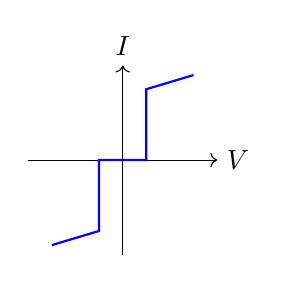
\begin{tikzpicture}[scale=0.6]
        \draw[->] (-2,0) -- (2,0) node[right] {$V$};
        \draw[->] (0,-2) -- (0,2) node[above] {$I$};
        \draw[thick, blue] (0,0) -- (0.5,0) -- (0.5,1.5) -- (1.5,1.8);
        \draw[thick, blue] (0,0) -- (-0.5,0) -- (-0.5,-1.5) -- (-1.5,-1.8);
    \end{tikzpicture} & 
    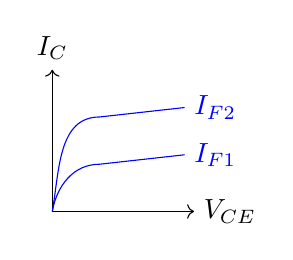
\begin{tikzpicture}[scale=0.6]
        \draw[->] (0,0) -- (3,0) node[right] {$V_{CE}$};
        \draw[->] (0,0) -- (0,3) node[above] {$I_C$};
        \draw[blue] (0,0) to[out=80, in=180] (1,1) -- (2.8,1.2) node[right] {$I_{F1}$};
        \draw[blue] (0,0) to[out=80, in=180] (1,2) -- (2.8,2.2) node[right] {$I_{F2}$};
    \end{tikzpicture} \\
    Linear relationship between LED current and photodetector current & Non-linear triggering response with threshold & Linear current transfer characteristic \\
    CTR (Current Transfer Ratio) is key parameter & Triggering occurs at specific current threshold & Collector current depends on base illumination \\
\end{tabulary}
\end{center}

\begin{itemize}
    \item \textbf{CTR (Current Transfer Ratio)}: Ratio of output current to input current
    \item \textbf{Trigger Current}: Minimum current needed to activate the device
    \item \textbf{Linearity}: How proportional the output is to the input light
\end{itemize}
\end{solutionbox}
\mnemonicbox{LTL - Light Transfers Like current flows -- Linear for isolators/transistors, Triggered for TRIACs}

\questionmarks{1}{b}{4}
\textbf{Describe working \& constructional features of IGBT.}

\begin{solutionbox}
\textbf{IGBT Structure and Operation:}

\begin{center}
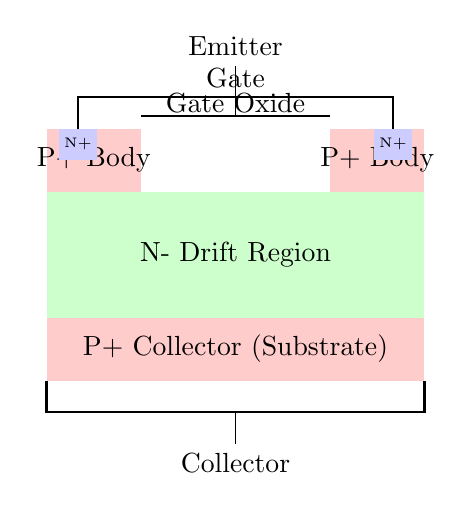
\begin{tikzpicture}[scale=0.8]
    % Layers
    \fill[fill=red!20] (0,0) rectangle (6,1); \node at (3,0.5) {P+ Collector (Substrate)};
    \fill[fill=green!20] (0,1) rectangle (6,3); \node at (3,2) {N- Drift Region};
    \fill[fill=red!20] (0,3) rectangle (1.5,4); \fill[fill=red!20] (4.5,3) rectangle (6,4);
    \node at (0.75,3.5) {P+ Body}; \node at (5.25,3.5) {P+ Body};
    \fill[fill=blue!20] (0.2,3.5) rectangle (0.8,4); \fill[fill=blue!20] (5.2,3.5) rectangle (5.8,4);
    \node at (0.5,3.75) {\tiny N+}; \node at (5.5,3.75) {\tiny N+};
    
    % Terminals
    \draw[thick] (0,0) -- (0,-0.5) -- (6,-0.5) -- (6,0); \draw (3,-0.5) -- (3,-1) node[below] {Collector};
    \draw[thick] (0.5,4) -- (0.5,4.5) -- (5.5,4.5) -- (5.5,4); \draw (3,4.5) -- (3,5) node[above] {Emitter};
    \draw[thick] (1.5,4.2) -- (4.5,4.2); \node at (3,4.4) {Gate Oxide};
    \draw (3,4.2) -- (3,4.5) node[above] {Gate};
\end{tikzpicture}
\end{center}

\begin{center}
\captionof{table}{IGBT Constructional Features}
\begin{tabulary}{\linewidth}{L L}
    \hline
    \textbf{Feature} & \textbf{Description} \\
    \hline
    Structure & Combines MOSFET input with BJT output \\
    Layers & Gate/Metal Oxide/P+ Body/N- Drift/P+ Collector \\
    Advantages & High input impedance, low conduction loss \\
    Switching & Faster than BJT, better power handling than MOSFET \\
    \hline
\end{tabulary}
\end{center}

\begin{itemize}
    \item \textbf{Voltage Controlled}: Device is controlled by gate voltage like MOSFET
    \item \textbf{Conductivity Modulation}: P+ collector injects holes into drift region
    \item \textbf{Low On-State Voltage}: Conduction losses lower than MOSFET
\end{itemize}
\end{solutionbox}
\mnemonicbox{IGBT MBC - Input from MOS, Body handles current, Collector acts like BJT}

\questionmarks{1}{c}{7}
\textbf{Explain working of SCR using two-transistor analogy.}

\begin{solutionbox}
\textbf{SCR as Two-Transistor Model:}

\begin{center}
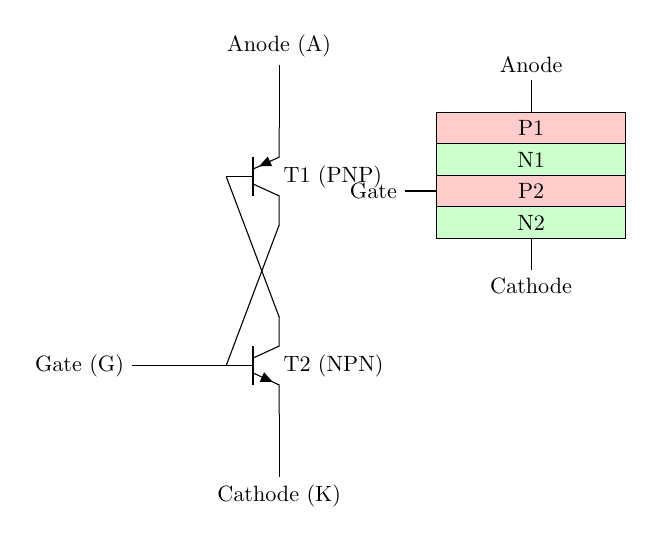
\begin{tikzpicture}[scale=0.8, transform shape]
    % PNP Transistor T1
    \draw (2,4) node[pnp, anchor=E] (T1) {T1 (PNP)};
    % NPN Transistor T2
    \draw (2,1) node[npn, anchor=C] (T2) {T2 (NPN)};

    % Connections
    \draw (T1.C) -- (T2.B);
    \draw (T1.B) -- (T2.C);
    
    % Terminals
    \draw (T1.E) -- ++(0,1) node[above] {Anode (A)};
    \draw (T2.E) -- ++(0,-1) node[below] {Cathode (K)};
    \draw (T2.B) -- ++(-1.5,0) node[left] {Gate (G)};
    
    % Block diagram representation
    \node[draw, fill=red!20, minimum width=3cm, minimum height=0.5cm] at (6,4) (P1) {P1};
    \node[draw, fill=green!20, minimum width=3cm, minimum height=0.5cm] at (6,3.5) (N1) {N1};
    \node[draw, fill=red!20, minimum width=3cm, minimum height=0.5cm] at (6,3) (P2) {P2};
    \node[draw, fill=green!20, minimum width=3cm, minimum height=0.5cm] at (6,2.5) (N2) {N2};
    
    \draw (P1.north) -- ++(0,0.5) node[above] {Anode};
    \draw (N2.south) -- ++(0,-0.5) node[below] {Cathode};
    \draw (P2.west) -- ++(-0.5,0) node[left] {Gate};
\end{tikzpicture}
\end{center}

\textbf{Two-Transistor Explanation:}

\begin{center}
\captionof{table}{SCR Two-Transistor Model Components}
\begin{tabulary}{\linewidth}{L L L}
    \hline
    \textbf{Component} & \textbf{Function} & \textbf{Connections} \\
    \hline
    PNP (T1) & Upper transistor & Emitter to Anode, Collector to N1, Base to P2-N1 junction \\
    NPN (T2) & Lower transistor & Emitter to Cathode, Collector to P1-N1 junction, Base to Gate \\
    Feedback & Regenerative action & T1's collector current = T2's base current \& vice versa \\
    \hline
\end{tabulary}
\end{center}

\begin{itemize}
    \item \textbf{Latching Mechanism}: Once triggered, transistors keep each other ON
    \item \textbf{Triggering}: Small gate current $\rightarrow$ T2 turns ON $\rightarrow$ T1 gets base current $\rightarrow$ Both remain ON
    \item \textbf{Holding Current}: Minimum current needed to maintain regenerative action
    \item \textbf{Turn-OFF}: Anode current must fall below holding current
\end{itemize}
\end{solutionbox}
\mnemonicbox{PPFF - Positive feedback Perpetuates Forward conduction}

\questionmarks{1}{c}{7}
\textbf{Explain the working of Solid state relay using Opto-SCR.}

\begin{solutionbox}
\textbf{Solid State Relay with Opto-SCR:}

\begin{center}
\begin{tikzpicture}[node distance=1.5cm, auto, >=stealth]
    \node[gtu block] (in) {AC/DC Input};
    \node[gtu block, right of=in, xshift=1.5cm] (led) {LED};
    \node[gtu block, right of=led, xshift=1.5cm] (photo) {Photo-SCR};
    \node[gtu block, right of=photo, xshift=1.5cm] (main) {Main SCR/TRIAC};
    \node[gtu block, right of=main, xshift=1.5cm] (load) {Load};
    
    \draw[gtu arrow] (in) -- (led);
    \draw[gtu arrow, dashed] (led) -- node[midway, above] {Light} (photo);
    \draw[gtu arrow] (photo) -- (main);
    \draw[gtu arrow] (main) -- (load);
    
    % Box for isolation
    \draw[dashed, red] (1.8,-1) rectangle (6,1);
    \node[red, below] at (4,-1) {Opto-Coupler Isolation};
\end{tikzpicture}
\end{center}

\textbf{Working Principle and Components:}

\begin{center}
\captionof{table}{Solid State Relay Stages and Functions}
\begin{tabulary}{\linewidth}{L L L}
    \hline
    \textbf{Stage} & \textbf{Function} & \textbf{Advantage} \\
    \hline
    Input & Low voltage control signal activates LED & Isolation from high power \\
    Opto-Coupler & LED light triggers photo-sensitive SCR & Electrical isolation \\
    Driver Circuit & Photo-SCR activates main switching device & Amplification of switching capacity \\
    Output Stage & Main SCR/TRIAC controls high-power load & Handles load current \\
    Snubber & RC circuit protects from voltage spikes & Prevents false triggering \\
    \hline
\end{tabulary}
\end{center}

\begin{itemize}
    \item \textbf{Electrical Isolation}: Complete separation between control and power circuits ($>1000$V)
    \item \textbf{Zero-Crossing}: Switching only at zero voltage reduces EMI/RFI noise
    \item \textbf{Silent Operation}: No mechanical clicks unlike traditional relays
    \item \textbf{Long Life}: No mechanical wear as in conventional relays
\end{itemize}
\end{solutionbox}
\mnemonicbox{LIPO - Light In, Power Out -- isolation guaranteed}

\questionmarks{2}{a}{3}
\textbf{Explain the working of snubber circuit for SCR.}

\begin{solutionbox}
\textbf{Snubber Circuit for SCR:}

\begin{center}
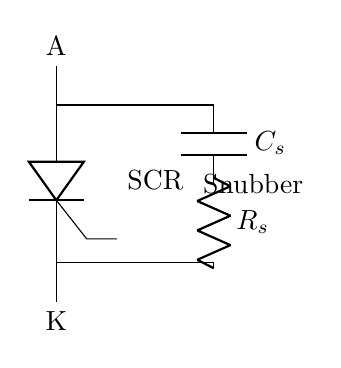
\begin{tikzpicture}
    % SCR
    \draw (0,0) to[thyristor, l=SCR] (0,-3);
    \draw (0,0) node[above] {A} -- (0,-0.5);
    \draw (0,-2.5) -- (0,-3) node[below] {K};
    
    % Snubber Branch
    \draw (0,-0.5) -- (2,-0.5) to[C, l=$C_s$] (2,-1.5) to[R, l=$R_s$] (2,-2.5) -- (0,-2.5);
    
    \node at (2.5, -1.5) {Snubber};
\end{tikzpicture}
\end{center}

\begin{center}
\captionof{table}{Snubber Circuit Components}
\begin{tabulary}{\linewidth}{L L L}
    \hline
    \textbf{Component} & \textbf{Purpose} & \textbf{Sizing Consideration} \\
    \hline
    Capacitor ($C_1$) & Limits $dv/dt$ rate & Based on max $dv/dt$ rating of SCR \\
    Resistor ($R_1$) & Limits discharge current & Based on capacitor value and switching frequency \\
    \hline
\end{tabulary}
\end{center}

\begin{itemize}
    \item \textbf{$dv/dt$ Protection}: Prevents false triggering due to rapid voltage rise
    \item \textbf{Turn-OFF Support}: Helps in commutation by providing alternate path
    \item \textbf{Energy Absorption}: Absorbs energy from inductive loads during switching
\end{itemize}
\end{solutionbox}
\mnemonicbox{CARD - Capacitor And Resistor Damp unwanted triggering}

\questionmarks{2}{b}{4}
\textbf{Write the differences between forced commutation and natural commutation.}

\begin{solutionbox}
\textbf{Comparison of Commutation Methods:}

\begin{center}
\captionof{table}{Forced vs Natural Commutation}
\begin{tabulary}{\linewidth}{L L L}
    \hline
    \textbf{Parameter} & \textbf{Forced Commutation} & \textbf{Natural Commutation} \\
    \hline
    Definition & External circuit forces SCR to turn OFF & AC source naturally reduces current to zero \\
    Application & DC circuits primarily & AC circuits primarily \\
    Components & Requires additional components (capacitors, inductors) & No extra components needed \\
    Complexity & More complex circuit design & Simpler circuit design \\
    Energy & Extra energy needed for commutation & Uses existing source energy \\
    Control & Can be controlled precisely & Happens at fixed points of AC cycle \\
    Cost & Higher due to extra components & Lower cost implementation \\
    \hline
\end{tabulary}
\end{center}

\begin{itemize}
    \item \textbf{Timing Control}: Forced commutation offers better timing control
    \item \textbf{Circuit Size}: Natural commutation results in smaller circuit size
    \item \textbf{Reliability}: Natural commutation has fewer components to fail
\end{itemize}
\end{solutionbox}
\mnemonicbox{DANCE - DC needs Active commutation, Natural for AC, Costs Extra for forced}

\questionmarks{2}{c}{7}
\textbf{Describe the working of UPS with the help of block diagram.}

\begin{solutionbox}
\textbf{UPS Block Diagram and Operation:}

\begin{center}
\begin{tikzpicture}[node distance=2cm, auto, >=stealth]
    % Nodes
    \node[gtu block] (ac) {AC Input};
    \node[gtu block, right of=ac, xshift=2cm] (rect) {Rectifier/Charger};
    \node[gtu block, below of=rect] (batt) {Battery Bank};
    \node[gtu block, right of=rect, xshift=2cm] (inv) {Inverter};
    \node[gtu block, right of=inv, xshift=1.5cm] (out) {Output Filter};
    \node[gtu block, right of=out, xshift=1.5cm] (load) {AC Output};
    \node[gtu block, above of=inv] (bypass) {Bypass Switch};

    % Connections
    \draw[gtu arrow] (ac) -- (rect);
    \draw[gtu arrow] (rect) -- (inv);
    \draw[gtu arrow] (inv) -- (out);
    \draw[gtu arrow] (out) -- (load);
    \draw[gtu arrow] (rect) -- (batt);
    \draw[gtu arrow] (batt) -- (inv);
    
    \draw[gtu arrow, dashed] (ac) |- (bypass);
    \draw[gtu arrow, dashed] (bypass) -| (load);
\end{tikzpicture}
\end{center}

\textbf{UPS Operation Modes:}

\begin{center}
\captionof{table}{UPS Operation Modes}
\begin{tabulary}{\linewidth}{L L L}
    \hline
    \textbf{Mode} & \textbf{Description} & \textbf{Power Path} \\
    \hline
    Normal & AC source powers load via rectifier and inverter & AC Input $\rightarrow$ Rectifier $\rightarrow$ Inverter $\rightarrow$ Output \\
    Battery & Battery powers load when AC fails & Battery $\rightarrow$ Inverter $\rightarrow$ Output \\
    Bypass & AC directly connects to load for maintenance & AC Input $\rightarrow$ Bypass Switch $\rightarrow$ Output \\
    Charging & Battery charges while in normal mode & Rectifier $\rightarrow$ Battery \\
    \hline
\end{tabulary}
\end{center}

\begin{itemize}
    \item \textbf{Online UPS}: Power always flows through rectifier/inverter (double conversion)
    \item \textbf{Offline UPS}: Power flows directly to load, switches to battery when power fails
    \item \textbf{Line-Interactive}: Similar to offline but with voltage regulation
    \item \textbf{Backup Time}: Depends on battery capacity and load requirements
\end{itemize}
\end{solutionbox}
\mnemonicbox{BRIC - Battery Ready when Input Cuts off}

\questionmarks{2}{a}{3}
\textbf{Explain pulse gate triggering method of SCR.}

\begin{solutionbox}
\textbf{Pulse Gate Triggering Method:}

\begin{center}
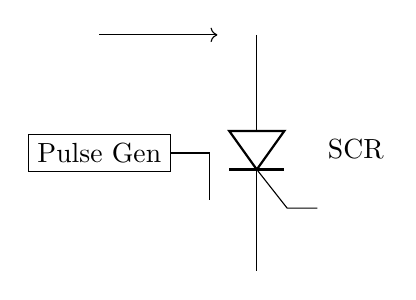
\begin{tikzpicture}
    \draw (0,0) to[thyristor, l=SCR] (0,-3);
    \node[draw] (pulse) at (-2,-1.5) {Pulse Gen};
    \draw (pulse.east) -- (-0.6,-1.5) -- (-0.6,-2.1); % Gate connection
    
    \draw[->] (-2,0) -- (-0.5,0); % Anode input
    
\end{tikzpicture}
\end{center}

\begin{center}
\captionof{table}{Pulse Gate Triggering Parameters}
\begin{tabulary}{\linewidth}{L L L}
    \hline
    \textbf{Parameter} & \textbf{Specification} & \textbf{Advantage} \\
    \hline
    Pulse Width & 10-100 $\mu$s & Ensures proper turn-on \\
    Amplitude & 1-3V above threshold & Reliable triggering \\
    Rise Time & Fast ($<1$ $\mu$s) & Quick turn-on \\
    Frequency & Single or train of pulses & Control over timing \\
    \hline
\end{tabulary}
\end{center}

\begin{itemize}
    \item \textbf{Precise Control}: Exact timing of SCR turn-on
    \item \textbf{Noise Immunity}: Less susceptible to false triggering
    \item \textbf{Power Efficiency}: Low average gate power consumption
    \item \textbf{Isolation}: Can be coupled through pulse transformer or opto-isolator
\end{itemize}
\end{solutionbox}
\mnemonicbox{TRAP - Timed, Reliable, Amplitude-controlled Pulses}

\questionmarks{2}{b}{4}
\textbf{List the commutation methods of SCR and explain any one in detail.}

\begin{solutionbox}
\textbf{Commutation Methods of SCR:}

\begin{center}
\captionof{table}{SCR Commutation Methods}
\begin{tabulary}{\linewidth}{L L L}
    \hline
    \textbf{Method} & \textbf{Circuit Type} & \textbf{Application} \\
    \hline
    Class A & Self-commutated by resonating LC & Low-power inverters \\
    Class B & Self-commutated by AC source & AC power control \\
    Class C & Complementary SCR commutation & DC choppers \\
    Class D & External pulse commutation & DC/AC converters \\
    Class E & External capacitor commutation & DC power control \\
    Class F & Line commutation & AC line controlled rectifiers \\
    \hline
\end{tabulary}
\end{center}

\textbf{Detailed Explanation of Class E (Capacitor Commutation):}

\begin{center}
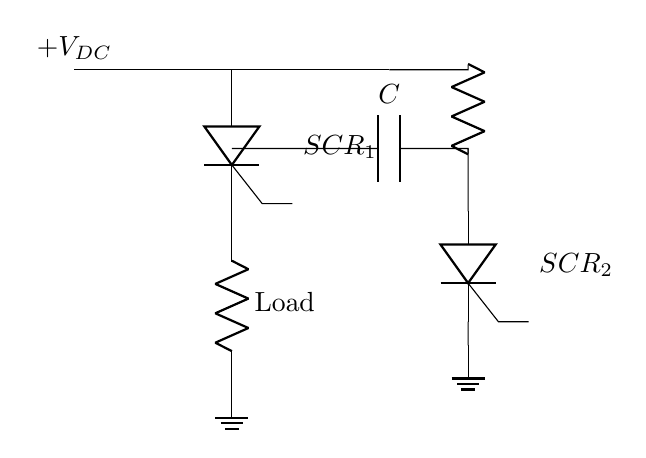
\begin{tikzpicture}
    % Main SCR1
    \draw (0,0) to[thyristor, l=$SCR_1$] (0,-2);
    % Load
    \draw (0,-2) to[R, l=Load] (0,-4) node[ground]{};
    % DC Source
    \draw (-2,0) node[above]{$+V_{DC}$} -- (2,0);
    
    % Commutation Circuit
    \draw (0,-1) -- (1,-1) to[C, l=$C$] (3,-1) -- (3,-1.5) to[thyristor, l=$SCR_2$] (3,-3.5) node[ground]{};
    \draw (2,0) -- (3,0) to[R] (3,-1); % Charging R for capacitor
\end{tikzpicture}
\end{center}

\begin{itemize}
    \item \textbf{Working Principle}: When $SCR_1$ is ON and carrying load current, firing $SCR_2$ connects pre-charged capacitor across $SCR_1$, reverse biasing it
    \item \textbf{Turn-OFF Time}: Determined by capacitor value and circuit resistance
    \item \textbf{Applications}: DC choppers, power control circuits, inverters
    \item \textbf{Advantages}: Simple circuit, reliable operation, cost-effective
\end{itemize}
\end{solutionbox}
\mnemonicbox{CARE - Capacitor Applies Reverse voltage for Extinction}

\questionmarks{2}{c}{7}
\textbf{Describe the working of SMPS with the help of block diagram.}

\begin{solutionbox}
\textbf{SMPS Block Diagram and Operation:}

\begin{center}
\begin{tikzpicture}[node distance=2.5cm, auto, >=stealth, scale=0.8, transform shape]
    \node[gtu block] (emif) {EMI Filter};
    \node[gtu block, right of=emif] (rect) {Rectifier/PFC};
    \node[gtu block, right of=rect] (inv) {HF Inverter};
    \node[gtu block, right of=inv] (trans) {HF Transformer};
    \node[gtu block, below of=trans] (outrect) {Rectifier/Filter};
    \node[gtu block, left of=outrect] (load) {Output DC};
    \node[gtu block, left of=load, xshift=-1cm] (ctrl) {Feedback/Control};
    
    \node[left of=emif] (in) {AC Input};

    \draw[gtu arrow] (in) -- (emif);
    \draw[gtu arrow] (emif) -- (rect);
    \draw[gtu arrow] (rect) -- (inv);
    \draw[gtu arrow] (inv) -- (trans);
    \draw[gtu arrow] (trans) -- (outrect);
    \draw[gtu arrow] (outrect) -- (load);
    
    \draw[gtu arrow] (load) -- (ctrl);
    \draw[gtu arrow] (ctrl) -| (inv);
    
\end{tikzpicture}
\end{center}

\textbf{SMPS Working Principles:}

\begin{center}
\captionof{table}{SMPS Block Functions}
\begin{tabulary}{\linewidth}{L L L}
    \hline
    \textbf{Block} & \textbf{Function} & \textbf{Key Components} \\
    \hline
    EMI Filter & Suppresses noise & Inductors, capacitors \\
    Rectifier/PFC & Converts AC to DC, improves power factor & Diodes, boost converter \\
    HF Inverter & Creates high-frequency AC & Switching transistors (MOSFET/IGBT) \\
    HF Transformer & Isolates and transforms voltage & Ferrite core transformer \\
    Output Stage & Rectifies and filters to clean DC & Fast diodes, LC filter \\
    Feedback & Regulates output voltage & Opto-isolator, PWM controller \\
    \hline
\end{tabulary}
\end{center}

\begin{itemize}
    \item \textbf{High Efficiency}: 70-95\% efficient compared to 50-60\% for linear power supplies
    \item \textbf{Size Reduction}: High-frequency operation allows smaller transformers
    \item \textbf{Regulation}: Feedback loop maintains stable output despite input/load changes
    \item \textbf{Protection}: Built-in overcurrent, overvoltage, and thermal protection
\end{itemize}
\end{solutionbox}
\mnemonicbox{RELIEF - Rectify, Energize at high frequency, Isolate, Extract DC, Feedback}

\questionmarks{3}{a}{3}
\textbf{State the method to protect SCR against over voltage.}

\begin{solutionbox}
\textbf{SCR Overvoltage Protection Methods:}

\begin{center}
\captionof{table}{SCR Overvoltage Protection Methods}
\begin{tabulary}{\linewidth}{L L L}
    \hline
    \textbf{Method} & \textbf{Circuit Implementation} & \textbf{Protection Level} \\
    \hline
    Snubber Circuit & RC network across SCR & $dv/dt$ protection \\
    MOV (Metal Oxide Varistor) & Connected across SCR & Transient suppression \\
    Voltage Clamping & Zener diodes in series & Fixed voltage limiting \\
    Crowbar Circuit & Sensing and shunting circuit & Complete shutdown \\
    \hline
\end{tabulary}
\end{center}

\begin{itemize}
    \item \textbf{Voltage Rating}: Always use SCR with voltage rating 2-3 times normal operating voltage
    \item \textbf{Rate-of-Rise}: Protect against fast transients with snubber circuits ($dv/dt$ protection)
    \item \textbf{Breakdown Voltage}: Never exceed reverse breakdown voltage of SCR junction
    \item \textbf{Coordinated Protection}: Use multiple methods for critical applications
\end{itemize}
\end{solutionbox}
\mnemonicbox{SCRAM - Snubber Circuits Reduce Abnormal Maximum voltages}

\questionmarks{3}{b}{4}
\textbf{State any four advantages of polyphase rectifiers over single-phase rectifiers.}

\begin{solutionbox}
\textbf{Advantages of Polyphase Rectifiers:}

\begin{center}
\captionof{table}{Polyphase Rectifier Advantages}
\begin{tabulary}{\linewidth}{L L L}
    \hline
    \textbf{Advantage} & \textbf{Explanation} & \textbf{Impact} \\
    \hline
    Higher Power Handling & Distributes load across phases & Suitable for high-power applications \\
    Reduced Ripple & Overlapping phases reduce output ripple & Less filtering required \\
    Better Transformer Utilization & Higher transformer utilization factor (0.955 vs 0.812) & More economical design \\
    Improved Power Factor & Better line utilization & Reduced line losses \\
    Lower Harmonic Content & Harmonics start at higher frequencies & Reduced EMI issues \\
    Higher Efficiency & Reduced losses due to better distribution & Lower operating costs \\
    \hline
\end{tabulary}
\end{center}

\begin{itemize}
    \item \textbf{Form Factor}: Lower form factor means better DC quality
    \item \textbf{Ripple Frequency}: Higher ripple frequency is easier to filter
    \item \textbf{Balanced Load}: Polyphase draws balanced current from supply
    \item \textbf{Size Reduction}: Smaller filter components needed
\end{itemize}
\end{solutionbox}
\mnemonicbox{HERBS - Higher efficiency, Even load, Reduced ripple, Better PF, Smaller filters}

\questionmarks{3}{c}{7}
\textbf{Describe the working of solar Photovoltaic (PV) based power generation with the help of block diagram.}

\begin{solutionbox}
\textbf{Solar PV Power Generation System:}

\begin{center}
\begin{tikzpicture}[node distance=2cm, auto, >=stealth]
    \node[gtu block] (pv) {Solar PV Array};
    \node[gtu block, right of=pv, xshift=1.5cm] (cc) {Charge Controller};
    \node[gtu block, right of=cc, xshift=1.5cm] (batt) {Battery Bank};
    \node[gtu block, below of=cc] (inv) {Inverter};
    \node[gtu block, left of=inv, xshift=-1cm] (acload) {AC Loads};
    \node[gtu block, right of=inv, xshift=1cm] (grid) {Grid};
    \node[gtu block, above of=cc] (mppt) {MPPT};

    \draw[gtu arrow] (pv) -- (cc);
    \draw[gtu arrow] (cc) -- (batt);
    \draw[gtu arrow] (batt) -- (inv);
    \draw[gtu arrow] (inv) -- (acload);
    \draw[gtu arrow] (inv) -- (grid);
    \draw[gtu arrow] (pv) -- (mppt);
    \draw[gtu arrow] (mppt) -- (cc);
\end{tikzpicture}
\end{center}

\textbf{System Components and Functions:}

\begin{center}
\captionof{table}{Solar PV System Components}
\begin{tabulary}{\linewidth}{L L L}
    \hline
    \textbf{Component} & \textbf{Function} & \textbf{Key Features} \\
    \hline
    PV Array & Converts sunlight to DC electricity & Multiple series/parallel connected panels \\
    MPPT & Maximizes power extraction & Tracks optimal operating point \\
    Charge Controller & Manages battery charging & Prevents overcharging/deep discharge \\
    Battery Bank & Energy storage & Deep cycle batteries for reliability \\
    Inverter & Converts DC to AC & Pure sine wave for sensitive equipment \\
    Distribution Panel & Routes power to loads & Includes protection devices \\
    \hline
\end{tabulary}
\end{center}

\begin{itemize}
    \item \textbf{Grid-Tied Systems}: Connected to utility grid, can sell excess power
    \item \textbf{Off-Grid Systems}: Standalone systems with battery storage
    \item \textbf{Hybrid Systems}: Can operate in both modes with battery backup
    \item \textbf{Efficiency}: Typical system efficiency 15-20\% from sunlight to usable electricity
\end{itemize}
\end{solutionbox}
\mnemonicbox{SIMPLE - Sun In, Maximum Power, Local Energy}

\questionmarks{3}{a}{3}
\textbf{State the method to protect SCR against over current.}

\begin{solutionbox}
\textbf{SCR Overcurrent Protection Methods:}

\begin{center}
\captionof{table}{SCR Overcurrent Protection Methods}
\begin{tabulary}{\linewidth}{L L L}
    \hline
    \textbf{Method} & \textbf{Implementation} & \textbf{Response Time} \\
    \hline
    Fuses & Fast-acting semiconductor fuses & Very fast (microseconds) \\
    Circuit Breakers & Magnetic/thermal breakers & Medium (milliseconds) \\
    Current Limiting Reactors & Series inductors & Instantaneous \\
    Electronic Current Limiting & Sensing and control circuits & Fast (microseconds) \\
    \hline
\end{tabulary}
\end{center}

\begin{itemize}
    \item \textbf{Current Rating}: Always use SCR with current rating above maximum operating current
    \item \textbf{di/dt Protection}: Limit rate of current rise to prevent junction damage
    \item \textbf{Thermal Management}: Proper heatsinking to prevent thermal runaway
    \item \textbf{Coordination}: Protection device must act before SCR is damaged
\end{itemize}
\end{solutionbox}
\mnemonicbox{FIRE - Fuses Immediately Restrict Excessive current}

\questionmarks{3}{b}{4}
\textbf{Explain basic principle of DC chopper.}

\begin{solutionbox}
\textbf{DC Chopper Basic Principle:}

\begin{center}
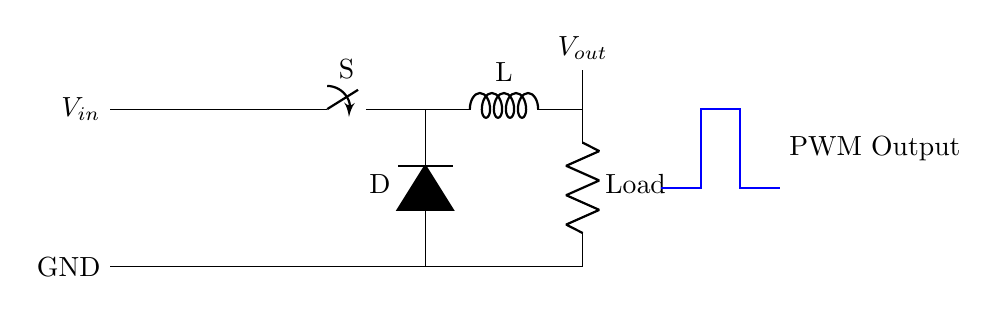
\begin{tikzpicture}
    % DC Input
    \draw (-2,2) node[left] {$V_{in}$} -- (0,2);
    \draw (-2,0) node[left] {GND} -- (0,0);
    
    % Switch
    \draw (0,2) to[switch, l=S] (2,2);
    
    % Diode and Inductor
    \draw (2,2) to[L, l=L] (4,2) to[R, l=Load] (4,0) -- (0,0);
    \draw (2,0) to[D*, l=D] (2,2); % Freewheeling Diode
    \draw (4,2) -- (4,2.5) node[above] {$V_{out}$};
    
    % Waveform hint
    \draw[blue, thick] (5,1) -- (5.5,1) -- (5.5,2) -- (6,2) -- (6,1) -- (6.5,1);
    \node[right] at (6.5, 1.5) {PWM Output};
\end{tikzpicture}
\end{center}

\begin{center}
\captionof{table}{DC Chopper Parameters}
\begin{tabulary}{\linewidth}{L L L}
    \hline
    \textbf{Parameter} & \textbf{Description} & \textbf{Effect} \\
    \hline
    Duty Cycle ($\alpha$) & Ratio of ON time to total period & Controls output voltage \\
    Switching Frequency & Number of ON/OFF cycles per second & Affects ripple and filter size \\
    Chopping Method & Step-up, Step-down, Buck-boost & Determines voltage conversion \\
    Control Strategy & PWM, Current mode, etc. & Affects system response \\
    \hline
\end{tabulary}
\end{center}

\begin{itemize}
    \item \textbf{Basic Equation}: $V_{out} = V_{in} \times$ Duty Cycle (for step-down chopper)
    \item \textbf{Operating Principle}: Rapid switching controls average voltage
    \item \textbf{Advantages}: High efficiency, precise control, compact size
    \item \textbf{Applications}: DC motor drives, battery charging, DC voltage regulation
\end{itemize}
\end{solutionbox}
\mnemonicbox{DISC - Duty cycle Influences Switching to Control output}

\questionmarks{3}{c}{7}
\textbf{Draw the circuit diagram of 3-$\Phi$ Full Wave rectifier using diode and explain it's working.}

\begin{solutionbox}
\textbf{3-Phase Full Wave Diode Rectifier (Bridge Configuration):}

\begin{center}
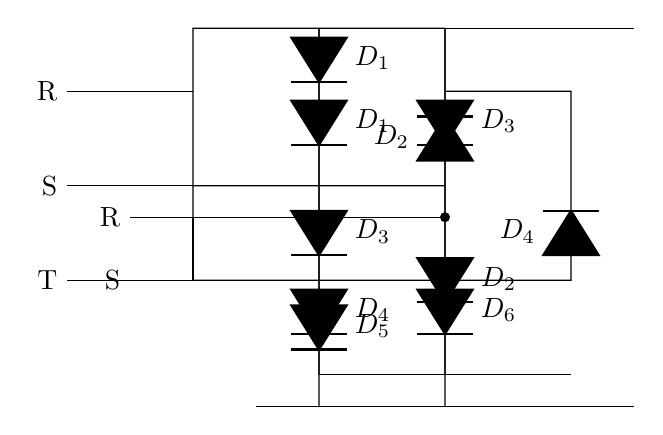
\begin{tikzpicture}[scale=0.8]
    % AC Setup
    \foreach \y/\l in {3/R, 1.5/S, 0/T} {
        \draw (-3,\y) node[left] {\l} -- (-1,\y);
    }
    
    % Bridge
    \draw (-1,3) -- (-1,4) -- (1,4) to[D*, l=$D_1$] (1,3);
    \draw (1,3) -- (1,1.5) to[D*, l=$D_3$] (1,0) to[D*, l=$D_5$] (1,-1.5);
    
    \draw (-1,3) -- (-1,1.5) -- (3,1.5) to[D*, l=$D_2$] (3,3) -- (3,4) -- (1,4); % Connect tops
    \draw (-1,1.5) -- (-1,0) -- (5,0) to[D*, l=$D_4$] (5,1.5) -- (5,3) -- (3,3); % Connect mid
    
    % Bottoms
    \draw (1,-1.5) -- (5,-1.5); % Common bottom rail
    \draw (3,1.5) to[D*, l=$D_2$] (3,-1.5); % Oops logic fix below
    
    % Let's redraw standard bridge logic
    % 3 legs: (D1, D4), (D3, D6), (D5, D2) ?
    % Standard 3-phase bridge:
    % Top rail, Bottom rail. 3 legs between them.
    % Leg 1: D1 top, D4 bottom. Input R to mid.
    % Leg 2: D3 top, D6 bottom. Input S to mid.
    % Leg 3: D5 top, D2 bottom. Input T to mid.
    
    \draw (0,4) -- (6,4); % Top DC+
    \draw (0,-2) -- (6,-2); % Bottom DC-
    
    % Leg 1
    \draw (1,4) to[D*, l=$D_1$] (1,1) node[circ]{} to[D*, l=$D_4$] (1,-2);
    \draw (-2,1) node[left] {R} -- (1,1);
    
    % Leg 2
    \draw (3,4) to[D*, l=$D_3$] (3,1) node[circ]{} to[D*, l=$D_6$] (3,-2);
    \draw (-2,0) node[left] {S} -- (-1,0) -- (-1,1) -- (3,1); % Visual fix needed, simple wires
    % Trying simple wires
\end{tikzpicture}

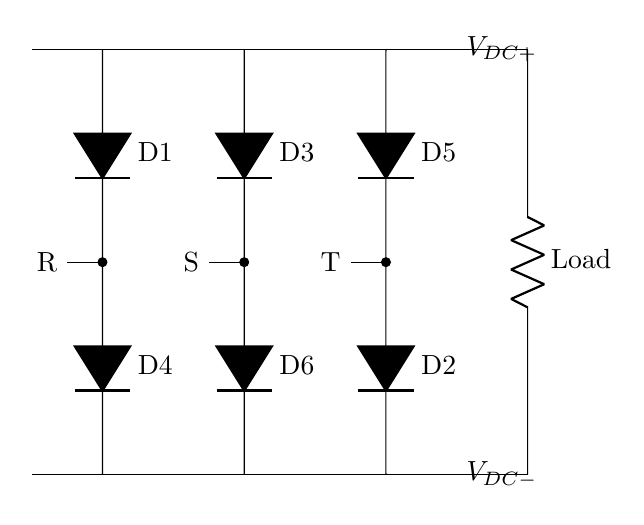
\begin{tikzpicture}[scale=0.9]
    % Top and Bottom Rails
    \draw (0,3) -- (6,3) node[right] {$V_{DC+}$};
    \draw (0,-3) -- (6,-3) node[right] {$V_{DC-}$};
    
    % Legs
    \foreach \x/\n/\t/\b in {1/R/D1/D4, 3/S/D3/D6, 5/T/D5/D2} {
        \draw (\x,3) to[D*, l=\t] (\x,0) to[D*, l=\b] (\x,-3);
        \draw (\x,0) node[circ]{} -- (\x-0.5,0) node[left] {\n};
    }
    
    % Load
    \draw (7,3) to[R, l=Load] (7,-3);
    \draw (6,3) -- (7,3);
    \draw (6,-3) -- (7,-3);
\end{tikzpicture}
\end{center}

\textbf{Working Principles:}

\begin{center}
\captionof{table}{3-Phase Rectifier Conduction Pattern}
\begin{tabulary}{\linewidth}{L L L}
    \hline
    \textbf{Phase} & \textbf{Conduction Pattern} & \textbf{Output Characteristics} \\
    \hline
    $0^\circ-60^\circ$ & D1 and D6 conduct & R and T phases connected to load \\
    $60^\circ-120^\circ$ & D1 and D2 conduct & R and S phases connected to load \\
    $120^\circ-180^\circ$ & D3 and D2 conduct & S and R phases connected to load \\
    $180^\circ-240^\circ$ & D3 and D4 conduct & S and T phases connected to load \\
    $240^\circ-300^\circ$ & D5 and D4 conduct & T and S phases connected to load \\
    $300^\circ-360^\circ$ & D5 and D6 conduct & T and R phases connected to load \\
    \hline
\end{tabulary}
\end{center}

\begin{itemize}
    \item \textbf{Ripple Frequency}: 6 times the input frequency (300/360Hz for 50/60Hz input)
    \item \textbf{Ripple Factor}: Approximately 4.2\% (much lower than single-phase)
    \item \textbf{Average Output Voltage}: $V_{dc} = 1.35 \times V_{rms}$ (line voltage)
    \item \textbf{Conduction Angle}: Each diode conducts for $120^\circ$ of cycle
\end{itemize}
\end{solutionbox}
\mnemonicbox{PRESTO - Pairs of diodes Rectify Efficiently, Six Times per cycle Output}

\questionmarks{4}{a}{3}
\textbf{Write the applications of Induction heating.}

\begin{solutionbox}
\textbf{Applications of Induction Heating:}

\begin{center}
\captionof{table}{Induction Heating Applications}
\begin{tabulary}{\linewidth}{L L L}
    \hline
    \textbf{Application Area} & \textbf{Specific Uses} & \textbf{Advantages} \\
    \hline
    Metal Heat Treatment & Hardening, annealing, tempering & Precise control, localized heating \\
    Melting & Foundry operations, precious metals & Clean, efficient melting \\
    Welding & Pipe welding, brazing, soldering & Concentrated heat, no contact \\
    Forging & Pre-heating billets, hot forming & Rapid heating, energy efficient \\
    Domestic & Induction cooktops & Safety, efficiency, control \\
    Medical & Hyperthermia treatment & Controlled deep tissue heating \\
    \hline
\end{tabulary}
\end{center}

\begin{itemize}
    \item \textbf{Industrial Advantages}: Fast heating, energy efficiency, clean process
    \item \textbf{Control Benefits}: Precise temperature control, repeatable results
    \item \textbf{Environmental Impact}: Reduced emissions compared to fossil fuel heating
    \item \textbf{Metallurgical Quality}: Improved material properties in many applications
\end{itemize}
\end{solutionbox}
\mnemonicbox{HAMMER - Hardening, Annealing, Melting, Medical, Eddy-current cooking, Reshaping metals}

\questionmarks{4}{b}{4}
\textbf{Draw and explain the circuit of controlling AC load using TRIAC and DIAC.}

\begin{solutionbox}
\textbf{AC Load Control with TRIAC and DIAC:}

\begin{center}
\begin{tikzpicture}
    % AC Source
    \draw (-3,2) node[left]{AC} -- (-2,2);
    \draw (-3,0) node[left]{AC} -- (4,0); % Line Neutral
    
    % Trigger Circuit
    \draw (-2,2) to[vR, l=$R_1$] (0,2) -- (0,1) to[C, l=$C_1$] (0,0);
    \draw (0,1) -- (1,1) to[D*, l=DIAC] (1.5,1) -- (1.5,0.5); % Gate
    
    % TRIAC
    \draw (1.5,2) to[Ttriac, l=TRIAC, n=T] (1.5,0); 
    \draw (1.5,0.5) -- (T.G);
    \draw (-2,2) -- (1.5,2);
    
    % Load
    \draw (1.5,2) -- (4,2) to[R, l=LOAD] (4,0);
\end{tikzpicture}
\end{center}

\begin{center}
\captionof{table}{TRIAC-DIAC Circuit Components}
\begin{tabulary}{\linewidth}{L L L}
    \hline
    \textbf{Component} & \textbf{Function} & \textbf{Effect on Circuit} \\
    \hline
    $R_1$ & Variable resistor & Controls charging rate of $C_1$ \\
    $C_1$ & Timing capacitor & Creates phase shift for triggering \\
    DIAC & Bi-directional trigger & Provides sharp triggering pulse \\
    TRIAC & Power control device & Controls current to load \\
    RC Network & Phase-shift network & Determines firing angle \\
    \hline
\end{tabulary}
\end{center}

\begin{itemize}
    \item \textbf{Phase Control}: Adjusting $R_1$ changes phase angle at which DIAC triggers
    \item \textbf{Power Control}: Varying firing angle controls average power to load
    \item \textbf{Bi-directional Control}: Works on both half-cycles of AC input
    \item \textbf{Applications}: Light dimmers, fan speed control, heater control
\end{itemize}
\end{solutionbox}
\mnemonicbox{CRAFT - Capacitor and Resistor Adjust Firing Time}

\questionmarks{4}{c}{7}
\textbf{Explain Spot Welding with Working and Applications.}

\begin{solutionbox}
\textbf{Spot Welding Process and Applications:}

\begin{center}
\begin{tikzpicture}[node distance=2.5cm, auto, >=stealth]
    \node[gtu state] (s1) {Position};
    \node[gtu state, right of=s1] (s2) {Contact};
    \node[gtu state, right of=s2] (s3) {Current};
    \node[gtu state, below of=s3] (s4) {Heat};
    \node[gtu state, left of=s4] (s5) {Weld};
    \node[gtu state, left of=s5] (s6) {Cooling};
    
    \draw[gtu arrow] (s1) -- (s2);
    \draw[gtu arrow] (s2) -- (s3);
    \draw[gtu arrow] (s3) -- (s4);
    \draw[gtu arrow] (s4) -- (s5);
    \draw[gtu arrow] (s5) -- (s6);
\end{tikzpicture}
\end{center}

\textbf{Spot Welding Working Principle:}

\begin{center}
\captionof{table}{Spot Welding Process Stages}
\begin{tabulary}{\linewidth}{L L L}
    \hline
    \textbf{Stage} & \textbf{Process} & \textbf{Parameters} \\
    \hline
    Setup & Material placed between electrodes & Sheet thickness, material type \\
    Contact & Electrodes apply pressure & 200-1000 pounds pressure \\
    Current Flow & High current passes through workpiece & 1000-100,000 amperes \\
    Heating & Resistance creates localized heating & Temperatures around 2500$^\circ$F \\
    Fusion & Material melts and forms nugget & 0.1-1 seconds duration \\
    Cooling & Pressure maintained during cooling & Electrode cooling important \\
    \hline
\end{tabulary}
\end{center}

\textbf{Applications of Spot Welding:}
\begin{itemize}
    \item \textbf{Automotive}: Car body assembly, sheet metal joining
    \item \textbf{Electronics}: Battery tabs, small component assembly
    \item \textbf{Appliances}: Refrigerators, washing machines, dishwashers
    \item \textbf{Aerospace}: Aircraft panel assembly, lightweight structures
\end{itemize}
\end{solutionbox}
\mnemonicbox{PCAFRI - Position, Compress, Apply current, Form nugget, Release after cooling, Inspect}

\questionmarks{4}{a}{3}
\textbf{Write the applications of Dielectric heating.}

\begin{solutionbox}
\textbf{Applications of Dielectric Heating:}

\begin{center}
\captionof{table}{Dielectric Heating Applications}
\begin{tabulary}{\linewidth}{L L L}
    \hline
    \textbf{Industry} & \textbf{Applications} & \textbf{Advantages} \\
    \hline
    Food Processing & Defrosting, cooking, pasteurization & Uniform heating, speed \\
    Wood Industry & Drying, glue curing, delamination & Reduced time, improved quality \\
    Textile & Drying yarns, fibers, finished goods & Energy efficiency, speed \\
    Plastics & Preheating, molding, welding & Uniform heating, no surface damage \\
    Pharmaceutical & Drying, sterilization & Controlled process, speed \\
    Paper & Drying, glue setting & Uniform moisture removal \\
    \hline
\end{tabulary}
\end{center}

\begin{itemize}
    \item \textbf{Process Benefits}: Volumetric heating (heats throughout, not just surface)
    \item \textbf{Speed Advantage}: Significantly faster than conventional heating
    \item \textbf{Quality Improvement}: More uniform heating, better product quality
    \item \textbf{Energy Efficiency}: Direct energy transfer to material
\end{itemize}
\end{solutionbox}
\mnemonicbox{FITPP - Food, Insulation drying, Textiles, Plastics, Pharmaceutical products}

\questionmarks{4}{b}{4}
\textbf{Write short note on SCR Delay timer.}

\begin{solutionbox}
\textbf{SCR Delay Timer:}

\begin{center}
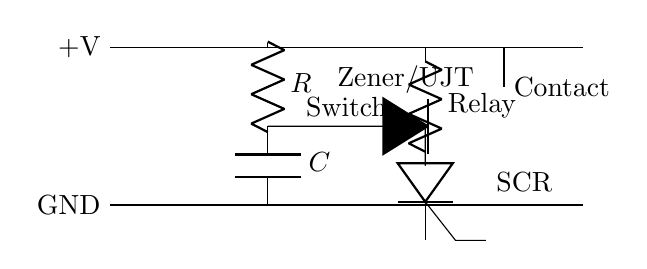
\begin{tikzpicture}
    % Supply
    \draw (-2,2) node[left]{+V} -- (4,2);
    \draw (-2,0) node[left]{GND} -- (4,0);
    
    % RC Timing
    \draw (0,2) to[R, l=$R$] (0,1) to[C, l=$C$] (0,0);
    \draw (0,1) -- (1,1) node[above]{Switch}; % Switch concept
    
    % Trigger
    \draw (0,1) -- (1.5,1) to[D*, l=Zener/UJT] (2,1) -- (2,0.5); % Simplified trigger
    
    % SCR
    \draw (2,2) to[R, l=Relay] (2,0.5) to[thyristor, l=SCR] (2,0);
    
    % Output
    \draw (3,2) -- (3,1.5) node[right]{Contact};
\end{tikzpicture}
\end{center}

\begin{center}
\captionof{table}{SCR Delay Timer Components}
\begin{tabulary}{\linewidth}{L L L}
    \hline
    \textbf{Component} & \textbf{Function} & \textbf{Selection Criteria} \\
    \hline
    RC Network & Determines time delay & $R \times C$ gives approximate timing \\
    SCR & Switching element & Current rating based on load \\
    UJT/Trigger & Provides gate pulse & Reliable triggering circuit \\
    Output Stage & Controls load & Relay or direct load connection \\
    \hline
\end{tabulary}
\end{center}

\begin{itemize}
    \item \textbf{Timing Principle}: RC charging time determines delay period
    \item \textbf{Accuracy}: Typically $\pm$5-10\% of set time
    \item \textbf{Applications}: Industrial process control, sequence control, protection circuits
    \item \textbf{Advantages}: Simple design, reliable operation, cost-effective
\end{itemize}
\end{solutionbox}
\mnemonicbox{TIME - Timing Is Managed by Electronics}

\questionmarks{4}{c}{7}
\textbf{Explain the working of SCR as static switch. Write the advantages of static switch.}

\begin{solutionbox}
\textbf{SCR as Static Switch:}

\begin{center}
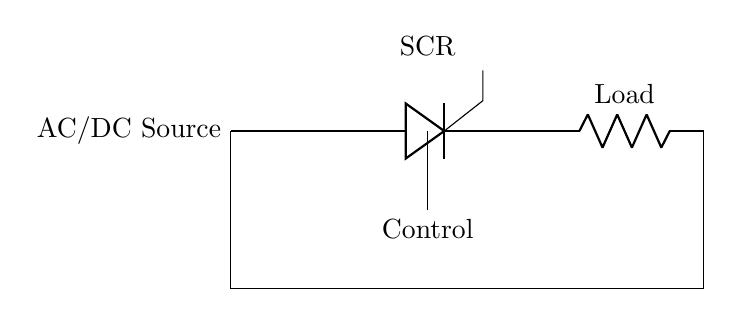
\begin{tikzpicture}
    \draw (0,0) node[left]{AC/DC Source} -- (1,0) to[thyristor, l=SCR] (4,0) to[R, l=Load] (6,0) -- (6,-2) -- (0,-2) -- (0,0);
    \draw (2.5,0) -- (2.5,-1) node[below]{Control};
\end{tikzpicture}
\end{center}

\textbf{Working Principles:}

\begin{center}
\captionof{table}{SCR Static Switch Operating Modes}
\begin{tabulary}{\linewidth}{L L L}
    \hline
    \textbf{Mode} & \textbf{State} & \textbf{Characteristics} \\
    \hline
    OFF State & No gate signal & High impedance, minimal leakage \\
    ON State & Gate triggered & Low impedance, high current flow \\
    Turn-ON & Gate pulse applied & Fast transition ($\mu$s range) \\
    Turn-OFF & Current falls below holding & Automatic in AC, needs commutation in DC \\
    \hline
\end{tabulary}
\end{center}

\textbf{Advantages of Static Switches:}

\begin{center}
\captionof{table}{Static Switch Advantages}
\begin{tabulary}{\linewidth}{L L L}
    \hline
    \textbf{Advantage} & \textbf{Description} & \textbf{Comparison with Mechanical} \\
    \hline
    No Moving Parts & No mechanical wear or tear & Longer lifetime (millions of operations) \\
    Silent Operation & No audible noise during switching & Important in noise-sensitive applications \\
    Fast Switching & Microsecond range switching & Much faster than mechanical contacts \\
    No Arcing & No contact bounce or arcing & Safer in hazardous environments \\
    Size \& Weight & Compact and lightweight & Significant space savings \\
    EMI/RFI & Less electromagnetic interference & Better for sensitive electronics \\
    \hline
\end{tabulary}
\end{center}
\end{solutionbox}
\mnemonicbox{FANS - Fast switching, Arc-free operation, No moving parts, Silent operation}

\questionmarks{5}{a}{3}
\textbf{What is DC Drive? Give Classification of DC Drives.}

\begin{solutionbox}
\textbf{DC Drive Definition and Classification:}

\begin{center}
\captionof{table}{DC Drive Definition}
\begin{tabulary}{\linewidth}{L L}
    \hline
    \textbf{Aspect} & \textbf{Description} \\
    \hline
    Definition & Electronic system that controls speed, torque, and direction of DC motors \\
    Basic Function & Controls armature voltage and/or field current to regulate motor parameters \\
    \hline
\end{tabulary}
\end{center}

\textbf{Classification of DC Drives:}

\begin{center}
\captionof{table}{DC Drives Classification}
\begin{tabulary}{\linewidth}{L L L}
    \hline
    \textbf{Classification Basis} & \textbf{Types} & \textbf{Characteristics} \\
    \hline
    Power Rating & Fractional, Integral, High Power & Based on horsepower rating \\
    Control Method & Open Loop, Closed Loop & Based on feedback mechanism \\
    Quadrant Operation & Single, Two, Four Quadrant & Based on speed/torque direction \\
    Power Supply & Single-phase, Three-phase & Based on input power configuration \\
    Converter Type & Half-wave, Full-wave, Chopper & Based on power conversion method \\
    Application & General Purpose, Servo, Specialized & Based on intended use \\
    \hline
\end{tabulary}
\end{center}

\begin{itemize}
    \item \textbf{Power Range}: From fractional HP to several thousand HP
    \item \textbf{Control Precision}: From basic to high-precision (0.01\%)
    \item \textbf{Response Time}: From milliseconds to microseconds
    \item \textbf{Protection}: Various built-in protection features
\end{itemize}
\end{solutionbox}
\mnemonicbox{PQCAS - Power rating, Quadrants, Control type, AC input phases, Switching method}

\questionmarks{5}{b}{4}
\textbf{Draw and explain the construction of variable reluctance type Stepper motor.}

\begin{solutionbox}
\textbf{Variable Reluctance Stepper Motor Construction:}

\begin{center}
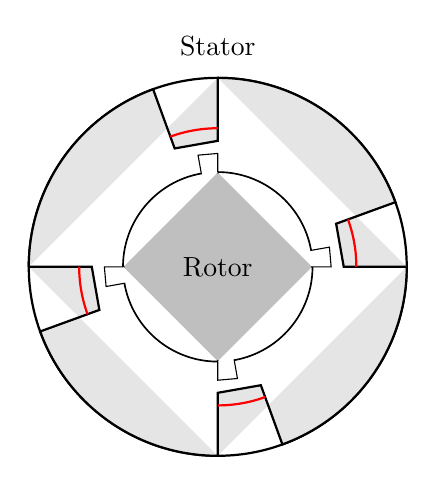
\begin{tikzpicture}[scale=0.8]
    % Stator
    \draw[thick] (0,0) circle (3cm);
    \foreach \a in {0, 90, 180, 270} {
        \draw[thick, fill=gray!20] (\a:3) -- (\a:2) -- (\a+20:2) -- (\a+20:3) arc (\a+20:\a+90:3);
        % Winding
        \draw[red, thick] (\a:2.2) arc (\a:\a+20:2.2);
    }
    
    % Rotor (Soft Iron)
    \draw[thick, fill=gray!50] (0,0) circle (1.5cm);
    \foreach \a in {0, 90, 180, 270} {
         \draw[fill=white] (\a:1.5) -- (\a:1.8) -- (\a+10:1.8) -- (\a+10:1.5) arc (\a+10:\a+90:1.5);
         % Rotor teeth usually different count, simplified here
    }
    \node at (0,0) {Rotor};
    \node at (0,3.5) {Stator};
\end{tikzpicture}
\end{center}

\begin{center}
\captionof{table}{Variable Reluctance Stepper Motor Components}
\begin{tabulary}{\linewidth}{L L L}
    \hline
    \textbf{Component} & \textbf{Construction} & \textbf{Function} \\
    \hline
    Stator & Laminated steel with multiple poles and windings & Creates magnetic field when energized \\
    Rotor & Soft iron with multiple teeth, NO permanent magnets & Aligns with energized stator poles \\
    Air Gap & Small space between rotor and stator & Affects step accuracy and torque \\
    Windings & Multiple phase windings on stator & Sequential energizing creates rotation \\
    \hline
\end{tabulary}
\end{center}

\begin{itemize}
    \item \textbf{Tooth Configuration}: Typically rotor teeth fewer than stator teeth
    \item \textbf{Step Angle}: Determined by: Step angle = $360^\circ \div$ (Number of rotor teeth $\times$ Number of phases)
    \item \textbf{Construction Simplicity}: No permanent magnets or windings on rotor
    \item \textbf{Operating Principle}: Magnetic reluctance path seeks to minimize when phases energized
\end{itemize}
\end{solutionbox}
\mnemonicbox{STAR - Stator energizes, Teeth Align with minimum Reluctance}

\questionmarks{5}{c}{7}
\textbf{Explain the working of VFD (Variable Frequency Drive).}

\begin{solutionbox}
\textbf{Variable Frequency Drive (VFD) Working:}

\begin{center}
\begin{tikzpicture}[node distance=2.5cm, auto, >=stealth, scale=0.8, transform shape]
    \node[gtu block] (rect) {Rectifier};
    \node[gtu block, right of=rect] (dcbus) {DC Bus/Filter};
    \node[gtu block, right of=dcbus] (inv) {Inverter};
    \node[gtu block, right of=inv] (motor) {AC Motor};
    
    \node[left of=rect] (ac) {AC Input};
    
    \node[gtu block, below of=dcbus] (ctrl) {Control System};
    \node[gtu block, left of=ctrl] (hmi) {HMI};
    \node[gtu block, right of=ctrl] (sense) {Sensors};
    
    \draw[gtu arrow] (ac) -- (rect);
    \draw[gtu arrow] (rect) -- (dcbus);
    \draw[gtu arrow] (dcbus) -- (inv);
    \draw[gtu arrow] (inv) -- (motor);
    
    \draw[gtu arrow] (ctrl) -- (rect);
    \draw[gtu arrow] (ctrl) -- (inv);
    \draw[gtu arrow] (hmi) -- (ctrl);
    \draw[gtu arrow] (sense) -- (ctrl);
\end{tikzpicture}
\end{center}

\textbf{VFD Components and Functions:}

\begin{center}
\captionof{table}{VFD Components and Functions}
\begin{tabulary}{\linewidth}{L L L}
    \hline
    \textbf{Component} & \textbf{Function} & \textbf{Features} \\
    \hline
    Rectifier & Converts AC to DC & 6-pulse or 12-pulse designs \\
    DC Bus & Filters and stores energy & Capacitors and inductors \\
    Inverter & Creates variable frequency AC & IGBT or MOSFET based \\
    Control System & Manages overall operation & Microprocessor based \\
    HMI & User interface & Display, keypad, communication \\
    Protection & System protection & Current, voltage, temperature sensors \\
    \hline
\end{tabulary}
\end{center}

\textbf{Working Principles:}

\begin{itemize}
    \item \textbf{Speed Control Equation}: Motor Speed (RPM) = (Frequency $\times$ 120) $\div$ Number of poles
    \item \textbf{Torque Control}: Maintaining V/F ratio controls torque output
    \item \textbf{Soft Start}: Gradual frequency/voltage ramp-up reduces inrush current
    \item \textbf{Braking Methods}: Regenerative, dynamic, or DC injection braking
    \item \textbf{Energy Savings}: Significant energy savings at reduced speeds
    \item \textbf{Advanced Features}: PID control, network communication, programmable functions
\end{itemize}
\end{solutionbox}
\mnemonicbox{DRIVE - DC conversion, Regulation, Inverter creates, Variable frequency, Efficient motor control}

\questionmarks{5}{a}{3}
\textbf{What are Hall effect sensors and what is their role in DC motors?}

\begin{solutionbox}
\textbf{Hall Effect Sensors in DC Motors:}

\begin{center}
\captionof{table}{Hall Effect Sensor Characteristics}
\begin{tabulary}{\linewidth}{L L}
    \hline
    \textbf{Aspect} & \textbf{Description} \\
    \hline
    Definition & Semiconductor-based sensors that detect magnetic fields \\
    Principle & Voltage difference generated perpendicular to current flow in magnetic field \\
    Signal Output & Digital (ON/OFF) or analog (proportional to field strength) \\
    Size & Compact, can be integrated into motor housing \\
    \hline
\end{tabulary}
\end{center}

\textbf{Role in DC Motors:}

\begin{center}
\captionof{table}{Hall Effect Sensor Role in DC Motors}
\begin{tabulary}{\linewidth}{L L L}
    \hline
    \textbf{Function} & \textbf{Application} & \textbf{Benefit} \\
    \hline
    Position Sensing & Rotor position detection & Precise commutation timing \\
    Speed Measurement & Pulse generation for RPM calculation & Accurate speed feedback \\
    Direction Detection & Phase sequence monitoring & Rotation direction control \\
    Current Sensing & Non-contact current measurement & Overload protection \\
    \hline
\end{tabulary}
\end{center}

\begin{itemize}
    \item \textbf{BLDC Motors}: Critical for electronic commutation (replacing mechanical commutator)
    \item \textbf{Precision}: Higher accuracy than mechanical sensors
    \item \textbf{Reliability}: No mechanical wear, longer service life
    \item \textbf{Integration}: Can be integrated with drive electronics
\end{itemize}
\end{solutionbox}
\mnemonicbox{MAPS - Measures position, Aids commutation, Provides speed data, Senses magnetic fields}

\questionmarks{5}{b}{4}
\textbf{Explain working principle of stepper motor.}

\begin{solutionbox}
\textbf{Stepper Motor Working Principle:}

\begin{center}
\begin{tikzpicture}[node distance=2cm, auto, >=stealth]
    \node[gtu state] (st1) {Phase A ON};
    \node[gtu state, right of=st1] (st2) {Phase B ON};
    \node[gtu state, below of=st2] (st3) {Phase C ON};
    \node[gtu state, left of=st3] (st4) {Phase D ON};
    
    \draw[gtu arrow] (st1) -- (st2);
    \draw[gtu arrow] (st2) -- (st3);
    \draw[gtu arrow] (st3) -- (st4);
    \draw[gtu arrow] (st4) -- (st1);
    
    \node[align=center] at (1, -1) {Rotor Alignment\\Cycle};
\end{tikzpicture}
\end{center}

\begin{center}
\captionof{table}{Stepper Motor Operating Modes}
\begin{tabulary}{\linewidth}{L L L}
    \hline
    \textbf{Operating Mode} & \textbf{Description} & \textbf{Advantages} \\
    \hline
    Full Step & One phase energized at a time & Maximum torque \\
    Half Step & Alternating one and two phases energized & Double resolution, smoother \\
    Microstepping & Proportional current in phases & Very smooth motion, high resolution \\
    Wave Drive & Sequential single phase energization & Lower power consumption \\
    \hline
\end{tabulary}
\end{center}

\begin{itemize}
    \item \textbf{Position Control}: Precise angular positioning without feedback
    \item \textbf{Step Angle}: Common step angles are 1.8$^\circ$ (200 steps/rev) or 0.9$^\circ$ (400 steps/rev)
    \item \textbf{Holding Torque}: Maintains position when phases energized at standstill
    \item \textbf{Open-Loop Control}: No position feedback normally required
    \item \textbf{Speed-Torque}: Torque decreases as speed increases
\end{itemize}
\end{solutionbox}
\mnemonicbox{STEPS - Sequential Triggering of Electromagnetic Phases causes Stepping}

\questionmarks{5}{c}{7}
\textbf{Draw the block diagram of PLC and explain the function of each block.}

\begin{solutionbox}
\textbf{PLC Block Diagram and Functions:}

\begin{center}
\begin{tikzpicture}[node distance=2cm, auto, >=stealth, scale=0.8, transform shape]
    \node[gtu block] (cpu) {CPU/Processor};
    \node[gtu block, left of=cpu, xshift=-1cm] (in) {Input Interface};
    \node[gtu block, right of=cpu, xshift=1cm] (out) {Output Interface};
    \node[gtu block, above of=cpu] (mem) {Memory};
    \node[gtu block, below of=cpu] (comm) {Communication};
    \node[gtu block, left of=mem] (ps) {Power Supply};
    \node[gtu block, right of=mem] (prog) {Programmer};
    
    \draw[gtu arrow] (ps) -- (cpu);
    \draw[gtu arrow] (in) -- (cpu);
    \draw[gtu arrow] (cpu) -- (out);
    \draw[gtu arrow] (cpu) -- (mem);
    \draw[gtu arrow] (mem) -- (cpu);
    \draw[gtu arrow] (prog) -- (cpu);
    \draw[gtu arrow] (comm) -- (cpu);
\end{tikzpicture}
\end{center}

\textbf{Functions of Each Block:}

\begin{center}
\captionof{table}{PLC Block Functions}
\begin{tabulary}{\linewidth}{L L L}
    \hline
    \textbf{Block} & \textbf{Function} & \textbf{Characteristics} \\
    \hline
    Power Supply & Converts main power to system voltages & Regulated, protected, with isolation \\
    CPU/Processor & Executes program, controls operations & Speed measured in scan time (ms) \\
    Input Interface & Connects to sensors and switches & Digital/analog, isolation, filtering \\
    Output Interface & Connects to actuators and indicators & Relay/transistor/triac outputs \\
    Memory & Stores program and data & Program, data, and system memory areas \\
    Programming Device & Used to develop and load programs & PC, handheld programmer, software \\
    Communication & Connects to networks/other devices & Industrial protocols, remote I/O \\
    \hline
\end{tabulary}
\end{center}

\begin{itemize}
    \item \textbf{Scan Cycle}: Sequential process of reading inputs, executing program, updating outputs
    \item \textbf{Programming Languages}: Ladder Diagram (LD), Function Block Diagram (FBD), Structured Text (ST), Instruction List (IL), Sequential Function Chart (SFC)
    \item \textbf{Modularity}: Expandable with additional I/O modules
    \item \textbf{Robustness}: Designed for harsh industrial environments
    \item \textbf{Reliability}: Typically MTBF $>100,000$ hours
\end{itemize}
\end{solutionbox}
\mnemonicbox{PICO MPC - Power, Inputs, CPU, Outputs, Memory, Programming interface, Communication}

\end{document}

